\documentclass[10pt,fleqn]{article}
% \usepackage[journal=rsc]{chemstyle}
% \usepackage{mhchem}
\usepackage{amsmath}
\usepackage{amssymb}
\usepackage{amsfonts}
\usepackage{esint}
\usepackage{bbm}
\usepackage{amscd}
\usepackage{picinpar}
\usepackage{graphicx}
\usepackage{tikz}
\usepackage{tikz-3dplot}
\usepackage{indentfirst}
\usepackage{wrapfig}
\usepackage{units}
\usepackage{textcomp}
\usepackage[utf8x]{inputenc}
% \usepackage{feyn}
\usepackage{feynmp}
\usepackage{xkeyval}
\usepackage{xargs}
\usepackage{verbatim}
\usepackage{pgfplots}
\usepackage{hyperref}
\usetikzlibrary{
  arrows,
  calc,
  decorations.pathmorphing,
  decorations.pathreplacing,
  decorations.markings,
  fadings,
  positioning,
  shapes
}

\DeclareGraphicsRule{*}{mps}{*}{}
\newcommand{\ud}{\mathrm{d}}
\newcommand{\ue}{\mathrm{e}}
\newcommand{\ui}{\mathrm{i}}
\newcommand{\res}{\mathrm{Res}}
\newcommand{\Tr}{\mathrm{Tr}}
\newcommand{\dsum}{\displaystyle\sum}
\newcommand{\dprod}{\displaystyle\prod}
\newcommand{\dlim}{\displaystyle\lim}
\newcommand{\dint}{\displaystyle\int}
\newcommand{\fsno}[1]{{\!\not\!{#1}}}
\newcommand{\eqar}[1]
{
  \begin{align}
    #1
  \end{align}
}
\newcommand{\texp}[2]{\ensuremath{{#1}\times10^{#2}}}
\newcommand{\dexp}[2]{\ensuremath{{#1}\cdot10^{#2}}}
\newcommand{\eval}[2]{{\left.{#1}\right|_{#2}}}
\newcommand{\paren}[1]{{\left({#1}\right)}}
\newcommand{\lparen}[1]{{\left({#1}\right.}}
\newcommand{\rparen}[1]{{\left.{#1}\right)}}
\newcommand{\abs}[1]{{\left|{#1}\right|}}
\newcommand{\sqr}[1]{{\left[{#1}\right]}}
\newcommand{\crly}[1]{{\left\{{#1}\right\}}}
\newcommand{\angl}[1]{{\left\langle{#1}\right\rangle}}
\newcommand{\tpdiff}[4][{}]{{\paren{\frac{\partial^{#1} {#2}}{\partial {#3}{}^{#1}}}_{#4}}}
\newcommand{\tpsdiff}[4][{}]{{\paren{\frac{\partial^{#1}}{\partial {#3}{}^{#1}}{#2}}_{#4}}}
\newcommand{\pdiff}[3][{}]{{\frac{\partial^{#1} {#2}}{\partial {#3}{}^{#1}}}}
\newcommand{\diff}[3][{}]{{\frac{\ud^{#1} {#2}}{\ud {#3}{}^{#1}}}}
\newcommand{\psdiff}[3][{}]{{\frac{\partial^{#1}}{\partial {#3}{}^{#1}} {#2}}}
\newcommand{\sdiff}[3][{}]{{\frac{\ud^{#1}}{\ud {#3}{}^{#1}} {#2}}}
\newcommand{\tpddiff}[4][{}]{{\left(\dfrac{\partial^{#1} {#2}}{\partial {#3}{}^{#1}}\right)_{#4}}}
\newcommand{\tpsddiff}[4][{}]{{\paren{\dfrac{\partial^{#1}}{\partial {#3}{}^{#1}}{#2}}_{#4}}}
\newcommand{\pddiff}[3][{}]{{\dfrac{\partial^{#1} {#2}}{\partial {#3}{}^{#1}}}}
\newcommand{\ddiff}[3][{}]{{\dfrac{\ud^{#1} {#2}}{\ud {#3}{}^{#1}}}}
\newcommand{\psddiff}[3][{}]{{\frac{\partial^{#1}}{\partial{}^{#1} {#3}} {#2}}}
\newcommand{\sddiff}[3][{}]{{\frac{\ud^{#1}}{\ud {#3}{}^{#1}} {#2}}}
\usepackage{fancyhdr}
\usepackage{multirow}
\usepackage{fontenc}
% \usepackage{tipa}
\usepackage{ulem}
\usepackage{color}
\usepackage{cancel}
\newcommand{\hcancel}[2][black]{\setbox0=\hbox{#2}%
  \rlap{\raisebox{.45\ht0}{\textcolor{#1}{\rule{\wd0}{1pt}}}}#2}
\pagestyle{fancy}
\setlength{\headheight}{67pt}
\fancyhead{}
\fancyfoot{}
\fancyfoot[C]{\thepage}
\fancyhead[R]{}
\renewcommand{\footruleskip}{0pt}
\renewcommand{\headrulewidth}{0.4pt}
\renewcommand{\footrulewidth}{0pt}

\newcommand\pgfmathsinandcos[3]{%
  \pgfmathsetmacro#1{sin(#3)}%
  \pgfmathsetmacro#2{cos(#3)}%
}
\newcommand\LongitudePlane[3][current plane]{%
  \pgfmathsinandcos\sinEl\cosEl{#2} % elevation
  \pgfmathsinandcos\sint\cost{#3} % azimuth
  \tikzset{#1/.estyle={cm={\cost,\sint*\sinEl,0,\cosEl,(0,0)}}}
}
\newcommand\LatitudePlane[3][current plane]{%
  \pgfmathsinandcos\sinEl\cosEl{#2} % elevation
  \pgfmathsinandcos\sint\cost{#3} % latitude
  \pgfmathsetmacro\yshift{\cosEl*\sint}
  \tikzset{#1/.estyle={cm={\cost,0,0,\cost*\sinEl,(0,\yshift)}}} %
}
\newcommand\DrawLongitudeCircle[2][1]{
  \LongitudePlane{\angEl}{#2}
  \tikzset{current plane/.prefix style={scale=#1}}
  % angle of "visibility"
  \pgfmathsetmacro\angVis{atan(sin(#2)*cos(\angEl)/sin(\angEl))} %
  \draw[current plane] (\angVis:1) arc (\angVis:\angVis+180:1);
  \draw[current plane,dashed] (\angVis-180:1) arc (\angVis-180:\angVis:1);
}
\newcommand\DrawLatitudeCircleArrow[2][1]{
  \LatitudePlane{\angEl}{#2}
  \tikzset{current plane/.prefix style={scale=#1}}
  \pgfmathsetmacro\sinVis{sin(#2)/cos(#2)*sin(\angEl)/cos(\angEl)}
  % angle of "visibility"
  \pgfmathsetmacro\angVis{asin(min(1,max(\sinVis,-1)))}
  \draw[current plane,decoration={markings, mark=at position 0.6 with {\arrow{<}}},postaction={decorate},line width=.6mm] (\angVis:1) arc (\angVis:-\angVis-180:1);
  \draw[current plane,dashed,line width=.6mm] (180-\angVis:1) arc (180-\angVis:\angVis:1);
}
\newcommand\DrawLatitudeCircle[2][1]{
  \LatitudePlane{\angEl}{#2}
  \tikzset{current plane/.prefix style={scale=#1}}
  \pgfmathsetmacro\sinVis{sin(#2)/cos(#2)*sin(\angEl)/cos(\angEl)}
  % angle of "visibility"
  \pgfmathsetmacro\angVis{asin(min(1,max(\sinVis,-1)))}
  \draw[current plane] (\angVis:1) arc (\angVis:-\angVis-180:1);
  \draw[current plane,dashed] (180-\angVis:1) arc (180-\angVis:\angVis:1);
}
\newcommand\coil[1]{
  {\rh * cos(\t * pi r)}, {\apart * (2 * #1 + \t) + \rv * sin(\t * pi r)}
}
\makeatletter
\define@key{DrawFromCenter}{style}[{->}]{
  \tikzset{DrawFromCenterPlane/.style={#1}}
}
\define@key{DrawFromCenter}{r}[1]{
  \def\@R{#1}
}
\define@key{DrawFromCenter}{center}[(0, 0)]{
  \def\@Center{#1}
}
\define@key{DrawFromCenter}{theta}[0]{
  \def\@Theta{#1}
}
\define@key{DrawFromCenter}{phi}[0]{
  \def\@Phi{#1}
}
\presetkeys{DrawFromCenter}{style, r, center, theta, phi}{}
\newcommand*\DrawFromCenter[1][]{
  \setkeys{DrawFromCenter}{#1}{
    \pgfmathsinandcos\sint\cost{\@Theta}
    \pgfmathsinandcos\sinp\cosp{\@Phi}
    \pgfmathsinandcos\sinA\cosA{\angEl}
    \pgfmathsetmacro\DX{\@R*\cost*\cosp}
    \pgfmathsetmacro\DY{\@R*(\cost*\sinp*\sinA+\sint*\cosA)}
    \draw[DrawFromCenterPlane] \@Center -- ++(\DX, \DY);
  }
}
\newcommand*\DrawFromCenterText[2][]{
  \setkeys{DrawFromCenter}{#1}{
    \pgfmathsinandcos\sint\cost{\@Theta}
    \pgfmathsinandcos\sinp\cosp{\@Phi}
    \pgfmathsinandcos\sinA\cosA{\angEl}
    \pgfmathsetmacro\DX{\@R*\cost*\cosp}
    \pgfmathsetmacro\DY{\@R*(\cost*\sinp*\sinA+\sint*\cosA)}
    \draw[DrawFromCenterPlane] \@Center -- ++(\DX, \DY) node {#2};
  }
}
\makeatother
\tikzstyle{snakearrow} = [decorate, decoration={pre length=0.2cm,
  post length=0.2cm, snake, amplitude=.4mm,
  segment length=2mm},thick, ->]
%% document-wide tikz options and styles
\tikzset{%
  >=latex, % option for nice arrows
  inner sep=0pt,%
  outer sep=2pt,%
  mark coordinate/.style={inner sep=0pt,outer sep=0pt,minimum size=3pt,
    fill=black,circle}%
}
\addtolength{\hoffset}{-1.3cm}
\addtolength{\voffset}{-2cm}
\addtolength{\textwidth}{3cm}
\addtolength{\textheight}{2.5cm}
\renewcommand{\footskip}{10pt}
\setlength{\headwidth}{\textwidth}
\setlength{\headsep}{20pt}
\setlength{\marginparwidth}{0pt}
\parindent=0pt
\title{Sideway circular polarization in tightly focused beam}

\ifpdf
  % Ensure reproducible output
  \pdfinfoomitdate=1
  \pdfsuppressptexinfo=-1
  \pdftrailerid{}
  \hypersetup{
    pdfcreator={},
    pdfproducer={}
  }
\fi

\begin{document}

\maketitle

\section{Goal}
Trying to accurately understand the origin of the sideway circular polarization
on the side of the focus of a tighly focused beam.\\

\section{Qualitative description}
For a collimated light beam, the polarization vector is generally within
the plane perpendicular to the wave propagation direction
(since light is a transverse wave).
However, for a focused beam, the ``wave propagation direction''
isn't very well defined anymore,
which allows polarization parallel to the optical axis to occur.
This ``axial'' polarization component could even lead to circular polarization
that rotates in a plane parallel to the optical axis, especially near the focus.\\

\begin{figure}[h]
  \centering
  \begin{tikzpicture}
    \draw[->,line width=1.5,red] (3, 3/2) -- +(-0.4, 0.8);
    \draw[->,line width=1.5,blue] (-3, 3/2) -- +(0.4, 0.8);

    \draw[->,line width=1.5,blue] (0, 0.4) -- +(0.4, 0.8);
    \draw[->,line width=1.5,red] (0, 0.4) -- +(-0.4, 0.8);

    \draw[->,line width=1.5,blue!50!red] ($(0, 1.6) + (-190:0.3 and 0.6)$(P) arc
    (-190:190:0.3 and 0.6);
    \draw[<-,line width=1.5,blue!50!red] ($(0, -1.6) + (-190:0.3 and 0.6)$(P) arc
    (-190:190:0.3 and 0.6);

    \draw[domain=-5:5,smooth,variable=\x,line width=2]
    plot ({\x}, {0.5 * sqrt((\x)^2 + 0.3)});
    \draw[domain=-5:5,smooth,variable=\x,line width=2]
    plot ({\x}, {-0.5 * sqrt((\x)^2 + 0.3)});
  \end{tikzpicture}
  \caption{Sideway circular polarization near the focus of a tighly focused beam.
    The red and blue error shows the polarization vector on the same edge
    of a tightly focused beam before and after the focus.}
  \label{fig:focus}
\end{figure}

We can qualitatively see this happening by looking at the field
on the edge of the beam.
The two edges have significantly different $k$ vectors
and therefore different polarization vectors as well.
As shown in Fig.~\ref{fig:focus}, the polarization on the two edges of the beam
acquires an axial component due to the large angle between the $k$ vector
and the optical axis. While the two sides of the beam are generally
far away from each other and their different polarization directions cause
little problem, this is not the case anymore near the focus as the edge of the beam
changes direction from converging to diverging and the polarization in that area
(next to the focus in the focal plane) would have a polarization somewhere in between.
This of course doesn't guarantee that there are any circular polarization
or even axial polarization component, which would be the topic of the next section.\\

\section{Semi-quantitative explanation}

Full quantitative understanding of the sideway circular polarization
near the focus of the beam requires a full calculation of the vector field.
It is possible, however, to understand why such a polarization exists
based on some continuity and symmetry considerations.\\

\subsection{General idea}
We can see from the far field (away from the focus)
that the axial polarization does exist~(Fig.~\ref{fig:focus}).
We can therefore break down the proof of the existance of
the sideway circular polarization in two steps.
\begin{enumerate}
\item Show that the axial polarization also exist on the focal plane.
\item Prove that the axial polarization has to be out-of-phase
  with the transverse polarization.
\end{enumerate}
These two would guarantee a sideway circular polarization.\\

\subsection{Existance of axial polarization on the focal plane}
\label{sec:semi:axial-pol}
Even though the three components of the electric field are related to one another,
they do all satisfy the scalar wave equation on their own~(Appendex~\ref{app:wave-eq}).
This allows us to consider the propagation of each components
independent of other ones.\\

\begin{figure}[h]
  \centering
  \begin{tikzpicture}
    \draw[->,line width=1.5,red] (3, 3/2) -- +(-0.4, 0.8);
    \draw[->,line width=1.5,blue] (-3, 3/2) -- +(0.4, 0.8);

    \draw[domain=-5:5,smooth,variable=\x,line width=2]
    plot ({\x}, {0.5 * sqrt((\x)^2 + 0.3)});
    \draw[domain=-5:5,smooth,variable=\x,line width=2]
    plot ({\x}, {-0.5 * sqrt((\x)^2 + 0.3)});

    \draw[->,line width=2] (-2.5, -3) -- node[above] {Wave propagation direction}
    (2.5, -3);

    \draw[dashed,line width=2] (-4, 2.5) node[above] {$P_0$} -- (-4, -2.5);
    \draw[dashed,line width=2] (0, 1.5) node[above] {$P_1$} -- (0, -1.5);

    \draw[->,line width=1.5] (-4.4, 1.2) node[left] {$\vec j_{\parallel}$} -- (-3.6, 1.2);
    \draw[->,line width=1.5] (-4.4, 0) node[left] {$\vec j_{\perp}$} -- (-3.6, 0);
    \draw[->,line width=1.5] (-4.4, -1.2) node[left] {$\vec j_{\parallel}$} -- (-3.6, -1.2);
  \end{tikzpicture}
  \caption{Scalar wave flux~(Appendix~\ref{app:wave-flux})
    for the transverse $\vec j_{\perp}$ and the longitudinal
    $\vec j_{\parallel}$ component of the field.
    In a plane far from the focus, $P_0$ we can verify that
    the flux for both components points to the right
    creating a net positive flux from left to right.
    For this reason, the net flux for both components should be non-null
    at all other parallel planes, including the focal plane $P_1$.}
  \label{fig:continuity}
\end{figure}

% TODO: plot the flux through P_0

For a traveling wave from left to right~(Fig.~\ref{fig:continuity}),
we can consider the flux of this scalar wave~(Appendix~\ref{app:wave-flux})
through a vertical plane. Since the flux is always in the direction
of the beam propagation (i.e. phase gradient), the net flux for both components
through a plane in the far field $P_0$ point to the right.
This means that the flux for both fields, and therefore the value of both fields
are non-null somewhere on the focal plane $P_1$.
We can therefore reasonably expect that there are points on the focal plane
where both fields are non-zero.\\

\subsection{Phase between the transverse and longitudinal polarization on the focal plane}
\label{sec:semi:axial-phase}
In this subsection we'll discuss a beam that's perfectly symmetric around
the focal plane.\footnote{I believe the existance of such field
  is a reasonably assumption to make, given the time reversal symmetry of EM field.}
More specifically, this means that the mirror reflection of the beam about
the focal plane should result in the same beam propagating backward
(i.e. mirror reflection plus time reversal should result in the same field).\\

\begin{figure}[h]
  \centering
  \begin{tikzpicture}
    \begin{scope}[shift={(-3, 0)}]
      \node[above] at (-1.5, 1.5) {Original};
      \node[above,align=center] at (1.5, 1.5) {Reflected and\\time reversed};
      \draw[dashed,line width=2] (0, 1.5) -- (0, -1.5);

      \draw[red,->,line width=2] (-1.5 - 0.2, 0.75 - 0.5) -- (-1.5 + 0.2, 0.75 + 0.5);
      \draw[blue,->,line width=2] (1.5 + 0.2, 0.75 - 0.5) -- (1.5 - 0.2, 0.75 + 0.5);

      \draw[red,->,line width=2] (-1.5 + 0.2, -0.75 - 0.5) -- (-1.5 - 0.2, -0.75 + 0.5);
      \draw[blue,->,line width=2] (1.5 - 0.2, -0.75 - 0.5) -- (1.5 + 0.2, -0.75 + 0.5);
    \end{scope}

    \begin{scope}[shift={(3, 0)}]
      \node[above] at (-1.5, 1.5) {Original};
      \node[above,align=center] at (1.5, 1.5) {Reflected and\\time reversed};
      \draw[dashed,line width=2] (0, 1.5) -- (0, -1.5);

      \draw[red,->,line width=2] ($(-1.5, 0.75) + (-190:0.2 and 0.5)$(P) arc
      (-190:195:0.2 and 0.5);
      \draw[blue,->,line width=2] ($(1.5, 0.75) + (-190:0.2 and 0.5)$(P) arc
      (-190:195:0.2 and 0.5);

      \draw[red,->,line width=2] ($(-1.5, -0.75) + (190:0.2 and 0.5)$(P) arc
      (190:-195:0.2 and 0.5);
      \draw[blue,->,line width=2] ($(1.5, -0.75) + (190:0.2 and 0.5)$(P) arc
      (190:-195:0.2 and 0.5);
    \end{scope}
  \end{tikzpicture}
  \caption{Time reversal and spacial reflection changes linear polarization
    that is not aligned with or perpendicular to the reflection plane (left).
    However, it will maintain an elliptical polarization
    if the axis of ellipse is straight (right).}
  \label{fig:symmetry}
\end{figure}
For a point on the focal plane with both longitudinal and transverse polarization
components, this require the polarization itself to be symmetric under
this transformation. Any in phase component between the two polarization directions
would break such symmetry. In fact, the symmetry is only preserved
if the two components are off by a phase $\pm\dfrac{\pi}{2}$,
or when the polarization is a straight ellipse~(Fig.~\ref{fig:symmetry}).\\

The result will of course not fully applicable to physical beam
without the perfect symmetry but the general result should still apply.
In another word, the point next to the focus on the focal plane may not have
a straight elliptical polarization (i.e. a perfectly out-of-phase axial compoment)
but the polarization should still be elliptical and the straight ellipse
may be achieved on a nearby plane/point.\\

\subsection{Approximate the axial polarization using Hermite-Gaussian modes}
In the far field, the wavefront of the axial polarization is approximately
$x \tilde A(x, y)$ where $\tilde A(x, y)$ is the wavefront for
the transverse polarization and we are assuming that the polarization is along $\hat x$.
Therefore, when the beam (i.e. the normal, transversely polarized portion)
is a Gaussian beam, the longitudinal polarization is approximately a $\mathrm{TEM}_{10}$
Gaussian mode
\footnote{\url{https://en.wikipedia.org/wiki/Gaussian_beam\#Hermite-Gaussian_modes}},
and we should be able to use it to check the properties we've predicted above~(Fig.~\ref{fig:hermite-gaussian}).\\

\begin{figure}[h]
  \centering
  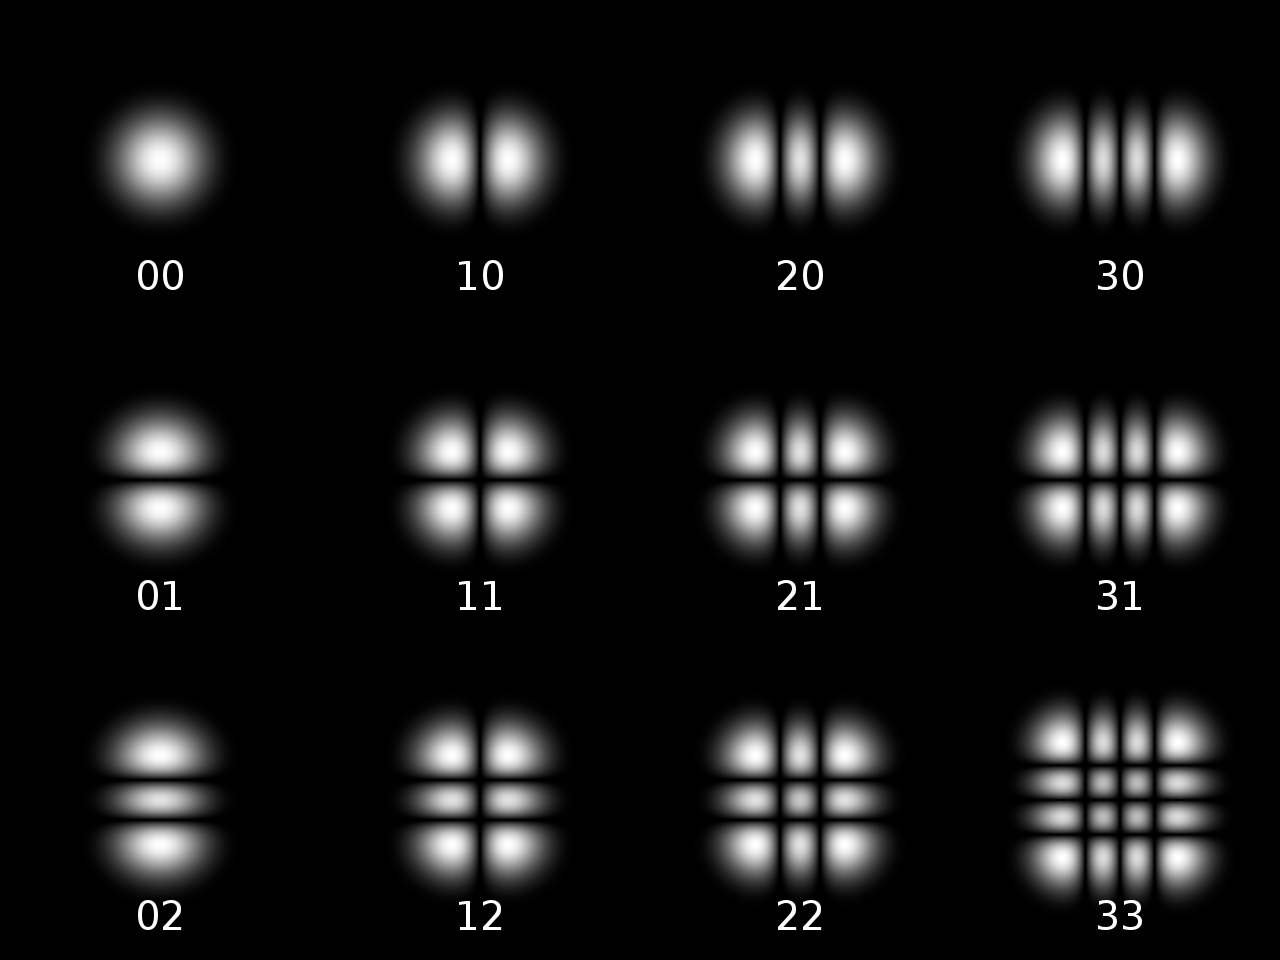
\includegraphics[width=8cm]{imgs/Hermite-gaussian.png}
  \caption{Power distribution of some Hermite Gaussian modes.
    The wavefront of the longitudinal polarization for a focused $\mathrm{TEM}_{00}$
    can be approximated by the $\mathrm{TEM}_{10}$ mode.}
  \label{fig:hermite-gaussian}
\end{figure}

Compared to the normal Gaussian beam (i.e. the $\mathrm{TEM}_{00}$ mode)
there are two main differences that we care about.
\begin{enumerate}
\item The amplitude profile of its wavefront is proportional to
  $x\ue^{-(x^2+y^2)/w^2}$ instead of $\ue^{-(x^2+y^2)/w^2}$
  for the normal ($\mathrm{TEM}_{00}$) mode.
  Note that the amplitude profile remains this shape and non-zero,
  which is consistent with our conclusion in section~\ref{sec:semi:axial-pol}.
\item The phase of the beam is different. Compared to a plain wave,
  which has a phase $\ue^{\ui kz}$ in the propagation direction,
  a focused beam picks up an additional phase, the so-called ``Gouy phase'',
  in the form $N\arctan\paren{z/z_R}$ where $z_R$ is the Rayleigh range of the beam.
  For the normal $\mathrm{TEM}_{00}$ mode, $N$ is $1$
  and for the $\mathrm{TEM}_{10}$ mode, $N$ is $2$.
  The longitudinal and transverse field are in phase in the far field
  and so they acquire a relative $\dfrac{\pi}{2}$ phase after propagating to the focus.
  This phase is exactly the same as the one we found in
  section~\ref{sec:semi:axial-phase},
  which explains the sideway elliptical polarization.
\end{enumerate}

\clearpage
\appendix
\section{Wave equation for electric field}
\label{app:wave-eq}
From the Maxwell equation,
\eqar{
  \begin{split}
    \nabla\times\paren{\nabla\times\vec E}=&-\nabla\times\pdiff{\vec B}{t}\\
    =&-\pdiff{\nabla\times\vec B}{t}\\
    =&-\frac{1}{c^2}\pdiff[2]{\vec E}{t}
  \end{split}\\
  \begin{split}
    \nabla\times\paren{\nabla\times\vec E}
    =&\nabla\paren{\nabla\cdot\vec E}-\nabla^2\vec E\\
    =&-\nabla^2\vec E
  \end{split}\\
  \nabla^2\vec E=&\frac{1}{c^2}\pdiff[2]{\vec E}{t}\label{app:eq:e-wave-eq}
}
Equation~\ref{app:eq:e-wave-eq} contains no mixing between the different components
of the electric field which shows that each compoments of the electric field
all satisfy the scalar wave equation.\\

\section{Continuity equation for scalar wave}
\label{app:wave-flux}
Consider a complex scalar wave $u(\vec r, t)$, it satisfy the wave equation,
\eqar{
  \nabla^2u=&\frac{1}{c^2}\pdiff[2]{u}{t}
}
If the wave is monotonic\footnote{
  We'll consider only a monotonic field to simplify the math but a time-dependenty
  continuity equation for a generic scalar wave also exists.},
we can write it out as $u(\vec r, t)=u_0(\vec r)\ue^{\ui\omega t}$,
in which case the wave equation becomes,
\eqar{
  \nabla^2u_0=&k^2 u_0
}
where the wave vector $k\equiv\dfrac{\omega}{c}$.
We can now define the flux of the wave $\vec j\equiv u_0^*\nabla u_0-u_0\nabla u_0^*$,
we have,
\eqar{
  \begin{split}
    \nabla\cdot\vec j=&\nabla\cdot\paren{u_0^*\nabla u_0-u_0\nabla u_0^*}\\
    =&\nabla u_0^*\cdot\nabla u_0-\nabla u_0\cdot\nabla u_0^*+u_0^*\nabla^2 u_0-u_0\nabla^2 u_0^*\\
    =&u_0^*k^2 u_0-u_0k^2 u_0^*\\
    =&0
  \end{split}
}
i.e. $\vec j$ is a continuous flow that cannot terminate in free space.

For a plane wave, this vector $\vec j$ points in the direction of the wave propagation.
Generically, this points in the direction of the phase gradient
(i.e. ``local'' propagation direction).\\

\end{document}
